% Preamble
\documentclass[12pt]{CLASS/protokol}
% --------

\usepackage{listings}
\usepackage{mathtools}

% Definice proměnných pro titulní stránku
% Přepište text v složených závorkách na požadované hodnoty
% např: {Datum měření} -> {1.1.1900}
\newcommand{\predmet}{Numerické metody}
\newcommand{\uloha}{ŘEŠENÍ SYSTÉMŮ ROVNIC S~TŘÍDIAGONÁLNÍMI MATICEMI}
\newcommand{\jmeno}{Lukáš Lev, 256660}
% -------------------------------------

%-----Bibliografie-----
\RequirePackage[backend=biber,style=iso-authoryear]{biblatex} % Nastavení citační normy na ISO 690:2022
\DefineBibliographyStrings{czech}{
  references = {Seznam použité literatury}, % Nastaví jméno referencí
}


\addbibresource{citace.bib} % Soubor s citacemi v BibLaTeXu

\definecolor{codegreen}{rgb}{0,0.6,0}
\definecolor{codegray}{rgb}{0.5,0.5,0.5}
\definecolor{codepurple}{rgb}{0.58,0,0.82}
\definecolor{backcolour}{rgb}{0.95,0.95,0.92}

\lstdefinestyle{mystyle}{
    backgroundcolor=\color{backcolour},
    commentstyle=\color{codegreen},
    keywordstyle=\color{magenta},
    numberstyle=\tiny\color{codegray},
    stringstyle=\color{codepurple},
    basicstyle=\ttfamily\footnotesize,
    breakatwhitespace=false,
    breaklines=true,
    captionpos=b,
    keepspaces=true,
    numbers=left,
    numbersep=5pt,
    showspaces=false,
    showstringspaces=false,
    showtabs=false,
    tabsize=2
}

\lstset{style=mystyle}


% Document
\begin{document}            % document start
\pagenumbering{gobble}      % číslování stránek
\pagenumbering{arabic}      % číslování stránek
\pagestyle{empty}           % bez číslování
%%%%%%%%%%%%%%%%%%%%%%%%%%%%%%%%%%%%%%%%%%%%%%%%%%%%%%%%%
%														%
%     Tuto Šablonu vytvořil Ing. Pavel Čudek, Ph.D.     %
%			pro potřeby předmětů DME a DIZ 				%
%														%
%%%%%%%%%%%%%%%%%%%%%%%%%%%%%%%%%%%%%%%%%%%%%%%%%%%%%%%%%
%                                                       %
% Tento soubor slouží ke generování titulní strany      %
% samostatné práce. Nic v tomto dokumentu neměňte.      %
% Titulnístrana se generuje automaticky z hodnot        %
% zadaných v souboru SP_Text.tex                        %
%                                                       %
%%%%%%%%%%%%%%%%%%%%%%%%%%%%%%%%%%%%%%%%%%%%%%%%%%%%%%%%%

\begin{titlepage}
    \end{titlepage}
	\begin{tikzpicture}[remember picture, overlay]
		\draw[line width = 2pt] ($(current page.north west) + (1cm,-1cm)$) rectangle ($(current page.south east) + (-1cm,1cm)$);
	\end{tikzpicture}

	\begin{center}
		\vspace{-1.5cm}

		\begin{figure}[!h]
            \centering
			
\includegraphics[width=8cm]{obrazky/UETE_Color_RGB_CZ.png}
		\end{figure}

		\vspace{3.5cm}

		{SAMOSTATNÁ PRÁCE Z PŘEDMĚTU}\\
		\vspace{0.25cm}

		\large{\textbf{\predmet}}\\
		\vspace{3.5cm}

		\textbf{NÁZEV PRÁCE: \uloha}
		\vspace{3cm}\\
		\vfill
        vypracoval: {\jmeno}
	\end{center}
\end{titlepage}  % Neměnit, odkaz na protokol_title.tex
\clearpage                  %
\setcounter{page}{2}        % Nastavení čísla druhé stránky na 2
\newpage                    % nová stránka (strana 2)

\section*{Anotace}          % Tady upravte anotaci
Na~základě zadání poskytnutého vyučujícím byla navržena a implementována metoda obdobná Gaussově eliminační metodě pro řešení třídiagonálních matic. Tato metoda byla testována na vzorovém příkladě (taktéž poskytnutém vyučujícím) a několika vlastních příkladech.

\newpage                    % Nová stránka (strana 3)
\tableofcontents            % Automaticky generovaný obsah
\newpage
\clearpage\pagestyle{plain} % Zapnout číslování stránek

\newcommand{\matice}[1]{\textbf{\textit{#1}}}

% Odsud dál pište text práce
% ==========================

\section{Zadání}\label{sec:zadani}
    Navrhněte a implementujte obdobu Gaussovy eliminační metody, která řeší soustavy s~třídiagonálními maticemi. Svůj program otestujte na soustavě (pro $n=100$):

    \begin{equation}\label{eq:zadani}
        \begin{bmatrix}   3 & -1 &  &  &  \\  -1 & 3 & -1 &  &  \\   & \ddots & \ddots & \ddots &  \\   &  & -1 & 3 & -1 \\   &  &  & -1 & 3\end{bmatrix} \cdot\begin{bmatrix}   x_1 \\ \\ \vdots \\ \\ x_n\end{bmatrix} =\begin{bmatrix}   2 \\ 1 \\ \vdots \\ 1 \\ 2\end{bmatrix}.
    \end{equation}



\section{Teorie a matematická metodika}\label{sec:teorie}
    \subsection{Třídiagonální matice}
        Třídiagonální matice jsou takové čtvercové matice, jejichž prvky mimo hlavní a~dvě první vedlejší diagonály nabývají nulové hodnoty. Tyto matice se v řešení numerických úloh vyskytují velmi často (např. při interpolaci pomocí splinových funkcí). Literatura běžně definuje tyto matice mají na zmíněných diagonálách nenulové prvky (\cite{Mika1985}), pro obecnější implementaci~v jazyce MATLAB však budeme pro účely této práce chápat třídiagonální matice z definice předchozí věty.

        \begin{equation}\label{eq:system}
            \matice{A}\vec{x} = \vec{b}
        \end{equation}

    \subsection{Thomasův algoritmus}
        Pro řešení systémů rovnic ve tvaru z rovnice \ref{eq:system} byl vybrán \textbf{Thomasův algoritmus} založený na separaci \matice{L} a \matice{U} matice coby složky matice \matice{A}. Protože vybírání hlavního prvku (dále nazývaného \uv{pivot}) by změnilo třídiagonální charakter matice \matice{A}, může dojít k dělení nulou i~když je \matice{A} regulární, nebo že výsledek výpočtu bude ovlivněn zaokrouhlováním (\cite{Rektorys1995}). Některé z těchto problémů jsou řešeny v~rámci implementace algoritmu v~jazyce MALTAB.
        \par
        Účelem Thomasova algoritmu je úpravami získat systém ve tvaru z rovnice \ref{eq:Upper} (pro rovnici \ref{eq:zadani}, kde $n=5$, viz \ref{eq:U+L}). Matice v tomto tvaru je někdy označována jako matice \matice{U} a~Thomasův algoritmus pak zprostředkovává tzv. LU faktorizaci (\cite{Rektorys1995}).
        \par
        K takovémuto tvaru lze dospět násobením koeficientem $m_i = a_{i-1} / b_{i-1}$, jež vychází z~prvků matice z~rovnice \ref{eq:U+L}. Dále jsou prvky matice a vektoru pravé strany $\vec{d}$ upravovány podle vztahů popsaných v rovnicích \ref{eq:koeficienty}, čímž je dosaženo kýženého stavu.
        \par
        Z~tohoto tvaru systému je pak výpočetně snadné vyjádřit řešení zpětnými substitucemi sestupně (nejdříve je vyjádřeno $x_5 = d'_5/b'5$ atd.).
        \par
        Během návrhu algoritmu bylo zváženo, zda nulovat prvky hlavní diagonály, což by zjednodušilo některé výpočty především při výpočtu člověkem. Protože je však algoritmus implementován do~počítače, byla tato varianta zavržena pro snížení počtu matematických operací, jež zvyšují zaokrouhlovací chybu.

        \begin{equation}\label{eq:U+L}
            \begin{bmatrix}
                b_1 & c_1 & 0 & 0 & 0 \\
                a_5 & b_2 & c'_2 & 0 & 0 \\
                0 & a_5 & b_3 & c'_3 & 0 \\
                0 & 0 & a_5 & b_4 & c_4 \\
                0 & 0 & 0 & a_5 & b_5
            \end{bmatrix} \cdot
            \begin{bmatrix}
                x_1 \\
                x_2 \\
                x_3 \\
                x_4 \\
                x_5
            \end{bmatrix}  =
            \begin{bmatrix}
                d_1 \\
                d_2 \\
                d_3 \\
                d_4 \\
                d_5
            \end{bmatrix}
        \end{equation}

        \begin{equation}\label{eq:Upper}
            \begin{bmatrix}
                b'_1 & c'_1 & 0 & 0 & 0 \\
                0 & b'_2 & c'_2 & 0 & 0 \\
                0 & 0 & b'_3 & c'_3 & 0 \\
                0 & 0 & 0 & b'_4 & c'_4 \\
                0 & 0 & 0 & 0 & b'_5
            \end{bmatrix} \cdot
            \begin{bmatrix}
                x_1 \\
                x_2 \\
                x_3 \\
                x_4 \\
                x_5
            \end{bmatrix}  =
            \begin{bmatrix}
                d'_1 \\
                d'_2 \\
                d'_3 \\
                d'_4 \\
                d'_5
            \end{bmatrix}
        \end{equation}

        \begin{equation}\label{eq:koeficienty}
            \begin{cases}
              b'_i=b_i−m\cdot c_{i−1}\\
              d'_i=d_i−m \cdot d_{i−1}
            \end{cases}
        \end{equation}


\section{Implementace v jazyce MATLAB}
    Algoritmus popsaný v kapitole \ref{sec:teorie} byl následně dle zadání implementován v~jazyce MATLAB. Tato implementace je obsažena v jednom zdrojovém souboru s~názvem \matice{llev\_projekt.m}.
    \par
    Součástí tohoto souboru je hlavička, deklarace vstupních proměnných, základní funkce a uživatelská část kódu s~voláním implementovaných funkcí. Implementace hlavní funkce pro řešení soustavy s třídiagonální maticí je součástí úryvku \ref{ls:mainfunkce} (tento úryvek ukazuje zjednodušenou formu implementace, v souboru \matice{llev\_projekt.m} jsou jejím obsahem i~další funkcionality).
    \par
    Dalšími dvěma použitými funkcemi jsou funkce pouze pomocného charakteru pro naplnění matice \matice{A} a vektoru $\vec{b}$ (viz rovnici \ref{eq:system}).
    \par
    Z~úryvku \ref{ls:mainfunkce} je patrné, že se s diagonálami matice zachází jako s vlastními vektory, což sice znamená vytvoření separátních proměnných (může být pozitivní z pohledu modularity kódu), zároveň to však umožňuje snazší manipulaci s jejími prvky. Zároveň v této implementaci nejsou nulovány prvky $a_i$ matice \matice{A} (viz rovnici \ref{eq:U+L}), tak jako v kapitole \ref{sec:teorie}. Je to z~důvodu snížení výpočetního času, jelikož se dále ve~funkci pro výpočet tyto prvky nepoužívají.
    \par
    Uživatel by pak implementované funkce volal způsobem uvedeným v úryvku \ref{ls:use}. Pokud by byl takový kód spuštěn, jeho výstupem by byla definice matice \matice{A}, jež by byla naplněna prvky o~hodnotě -1 na~prvních vedlejších diagonálách a~prvky s~hodnotou 3 nebo 4, symetricky se střídající. Vektor pravých stran $\vec{b}$ by byl zase symetricky naplněn čísly 2 a 1. Takovéto volání odpovídá příkladu ze zadání (kapitola \ref{sec:zadani}), ovšem pro $n=10$.
    \par
    Celý kód je přiložen na straně \pageref{ls:uf}.

    \newpage
    \begin{lstlisting}[language=MATLAB,label=ls:use,caption=Příklad uživatelského volání funkcí implementovaných v souboru \matice{llev\_projekt.m}]
%% uzivatelska cast kodu
% soustava ze zadani
A = fill_diagonal(A,-1,[3;4],-1);
b = fill_rhsvector(b,[2;1],true);

% % reseni vlastni soustavy - test
% A = fill_diagonal(A,2,1,2);
% b = fill_rhsvector(b,[3;2],true);

disp(A);  % kontrola vstupu
disp(b);  % kontrola vstupu

x = solve_tridiagonal(A,b);  % volani funkce pro reseni

disp(x);  % kontrola vystupu
    \end{lstlisting}

    \begin{figure}
        \centering
        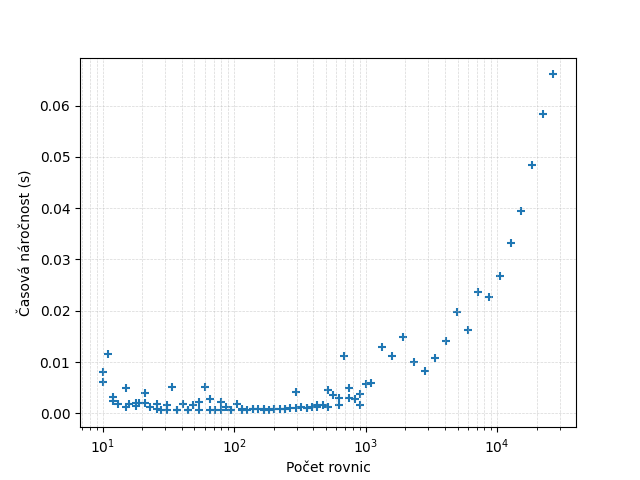
\includegraphics[width=1\linewidth]{obrazky/casova_narocnost.png}
        \caption{Závislost časové složitosti algoritmu na počtu rovnic}
        \label{fig:slozitost}
    \end{figure}

    \newpage
    \begin{lstlisting}[language=MATLAB, caption=Implementace funkce pro řešení třídiagonální matice v jazyce MATLAB, label=ls:mainfunkce]
function x = solve_tridiagonal(A, b)
    % ARGUMENTY:
    %   A ... tridiagonalni matice
    %   b ... vektor pravych stran

    n = length(b);  % pocet rovnic
    x = zeros(n,1);  % vystupni vektor

    % rozpoznani diagonal
    diag_mid = zeros(n,1);
    diag_low = zeros(n-1,1);
    diag_high = zeros(n-1,1);
    for i = 1:n
        diag_mid(i) = A(i,i);
        if i > 1
            diag_low(i) = A(i,i-1);
        end
        if i < n
            diag_high(i) = A(i,i+1);
        end
    end

    % eliminace prvku
    for i = 2:n
        if diag_mid(i-1) == 0  % zpetna kontrola pivotu
            error('System is not solvable: zero pivot at row %d', i-1);
        end
        m = diag_low(i-1) / diag_mid(i-1);  % multiplikator
        diag_mid(i) = diag_mid(i) - m * diag_high(i-1);  % eliminace
        b(i) = b(i) - m * b(i-1);  % aktualizace vektoru p. strany
    end

    % kontrola pivotu pro resitelnost
    if diag_mid(n) == 0
        error('System is not solvable: zero pivot at last row.');
    end

    % zpetna substituce
    x(n) = b(n) / diag_mid(n);
    for i = n-1:-1:1  % dekrementace i od poctu radku po 1
        if diag_mid(i) == 0  % overeni resitelnosti
            error('System is not solvable: zero pivot at row %d', i);
        end

        % zapis vysledku
        x(i) = (b(i) - diag_high(i) * x(i+1)) / diag_mid(i);
    end
end
    \end{lstlisting}

\section{Zpracování}
    Podle zadání byla implementace testována pro počet rovnic $n=100$, kde se v~porovnání s~analytickým řešením projevila jako spolehlivá (ačkoliv vykazuje asymetrie mezi oběma konci vektoru neznámých v~řádu desetin pro hodnoty ze~zadání).
    \par
    Zároveň byla testována časová složitost algoritmu, jež by bylo možno vyhodnotit jako $\mathcal{O}(n)$ podle grafu z obrázku \ref{fig:slozitost}. Je také třeba brát v potaz, že během měření časové složitosti není separován čas pro naplnění matice a vektoru pravé strany od času pro vlastní řešení systému, což může způsobit zkreslení.
    \par
    Zpracování této závislosti probíhá za~pomocí vlastního kódu, který není součástí souboru v~\matice{llev\_projekt.m} (viz \href{https://github.com/levlukas/2NU_projekt}{GitHub repozitář}).


\section{Závěr}
    V~rámci semestrální práce byla navržena metoda obdobná Gaussově eliminační metodě v~kapitole \ref{sec:teorie}. Tato metoda je založena na separaci matice \matice{L} a~\matice{U}, někdy je také nazývána Tomasovým algoritmem. Některé nedostatky tohoto algoritmu byly ošetřeny v~implementaci v~jazyce MATLAB.
    \par
    Samotná implementace pak byla obsahem jednoho souboru, jež je přiložen k~řešení. Nejdůležitější částí tohoto souboru je implementace funkce \uv{solve\_tridiagonal}, která je blíže zdokumentována v~úryvku \ref{ls:mainfunkce}.
    \par
    Nakonec byla implementována metoda srovnána s analytickými výsledky a byla vyjádřena její časová složitost. Empiricky vyhodnocená složitost $\mathcal{O}(n)$ je překvapivá v kontextu dvoudimenzionálních matic (předpokládala by se složitost $\Omega(n^2)$). Tato vlastnost je však důsledkem pásového charakteru matice.

\printbibliography

\newpage
\begin{lstlisting}[language=MATLAB,label=ls:uf]
%% ===== 2NU, semestralni projekt =====
% Zadani:
% Navrhnete a implementujte obdobu Gaussovy eliminacni metody, ktera
% resi soustavz s tridiagonalnimi maticemi.
%
% Autor:
% Lukas Lev, 2566660

%% Deklarace
n = 100;  % pocet rovnic
A = zeros(n);  % vstupni matice
b = zeros(n,1);


%% Funkce pro plneni diagonaly
% temp: naplneni diagonaly jen jednim cislem
function A = fill_diagonal(A,fill_low,fill_mid,fill_high,symmetric)
    % ARGUMENTY:
    %   A         ... vstupni matice
    %   fill_low  ... cislo / vektor pro vyplneni prvni vedlejsi diagonaly
    %                 pod hlavni
    %   fill_mid  ... cislo / vektor pro vyplneni hlavni diagonaly
    %   fill_high ... cislo / vektor pro vyplneni prvni vedlejsi diagonaly
    %                 nad hlavni
    %   symmetric ... nepovinne, pro naplneni symetricky

    % kontrola vstupu
    if ~ismatrix(A) && not(size(A,1) == size(1,A))
        error('Error: Input must be a square matrix.\n');
    end

    % pokud je vstupem cislo, napln nim vektor pro modularni naplneni
    % matice
    if ~isvector(fill_mid) & isnumeric(fill_mid)
        fill_mid = fill_mid(:);
    end
    if ~isvector(fill_low) & isnumeric(fill_low)
        fill_low = fill_low(:);
    end
    if ~isvector(fill_high) & isnumeric(fill_high)
        fill_high = fill_high(:);
    end
    if not(isvector(fill_high) || isvector(fill_low) || isvector(fill_mid))
        error('Error: Input must be numeric.\n');
    end

    % kontrola symetrie
    if nargin < 5
        symmetric = false;
    end

    % naplneni matice
    A = zeros(size(A));
    for i = 1:size(A)
        if symmetric
            idx = min(i, size(A) - i + 1);  % zaruceni symetrie
        else
            idx = i;
        end
        A(i, i) = fill_mid(mod(idx-1, length(fill_mid)) + 1);
        if i > 1
            A(i, i-1) = fill_low(mod(idx-2, length(fill_low)) + 1);
        end
        if i < size(A)
            A(i, i+1) = fill_high(mod(idx-1, length(fill_high)) + 1);
        end
    end
end


%% Funkce pro naplneni vektoru prave strany
function b = fill_rhsvector(b,fill,symmetric)
    % ARGUMENTY:
    %   b         ... vstupni vektor
    %   fill      ... cislo / vektor pro vyplneni vektoru prave strany
    %   symmetric ... nepovinne, pro naplneni symetricky

    % kontrola vstupu
    if ~isvector(b)
        error('Error: Input must be a vector.\n');
    end
    if ~isvector(fill) & isnumeric(fill)
        fill = fill(:);
    elseif ~isvector(fill)
        error('Error: Input must be numeric.\n');
    end

    % kontrola symetrie
    if nargin < 3
        symmetric = false;
    end

    % naplneni vektoru
    for i = 1:length(b)
        if symmetric
                idx = min(i, length(b)-i+1);  % zaruceni symetri
        else
            idx = i;
        end
        b(i) = fill(mod(idx-1, length(fill)) + 1);
    end
end


% Funkce pro reseni systemu
function x = solve_tridiagonal(A, b)
    % ARGUMENTY:
    %   A         ... tridiagonalni matice
    %   b         ... vektor pravych stran

    % kontrola vstupu
    if ~isvector(b)
        error('Error: Input must be a vector.\n');
    end
    if ~ismatrix(A)
        error('Error: Input must be a matrix.\n')
    end

    n = length(b);
    x = zeros(n,1);

    % rozpoznani diagonal
    diag_mid = zeros(n,1);
    diag_low = zeros(n-1,1);
    diag_high = zeros(n-1,1);
    for i = 1:n
        diag_mid(i) = A(i,i);
        if i > 1
            diag_low(i) = A(i,i-1);
        end
        if i < n
            diag_high(i) = A(i,i+1);
        end
    end

    % eliminace prvku
    for i = 2:n
        if diag_mid(i-1) == 0  % zpetna kontrola pivotu
            error('System is not solvable: zero pivot at row %d', i-1);
        end
        m = diag_low(i-1) / diag_mid(i-1);  % multiplikator pro aktualni radek
        diag_mid(i) = diag_mid(i) - m * diag_high(i-1);  % eliminace pod pivotem
        b(i) = b(i) - m * b(i-1);  % aktualizace vektoru p. strany
    end

    % kontrola pivotu pro resitelnost
    if diag_mid(n) == 0
        error('System is not solvable: zero pivot at last row.');
    end

    % zpetna substituce
    x(n) = b(n) / diag_mid(n);
    for i = n-1:-1:1  % dekrementace i od poctu radku po 1
        if diag_mid(i) == 0  % overeni resitelnosti
            error('System is not solvable: zero pivot at row %d', i);
        end

        % zapis vysledku
        x(i) = (b(i) - diag_high(i) * x(i+1)) / diag_mid(i);
    end
end


% %% Vyhodnoceni casove narocnosti
% filename = 'casova_narocnost.csv';
%
% % hlavicka csv
% if exist(filename, 'file') ~= 2
%     writetable(table("n", "elapsedTime"), filename, 'WriteVariableNames', false);
% end
%
% for n = logspace(1, 3)
%     n = round(n);  % n je cele cislo
%
%     A = zeros(n);  % reset promennych
%     b = zeros(n,1);
%
%     tic  % mereni casu
%         A = fill_diagonal(A, -1, [3;4], -1);
%         b = fill_rhsvector(b, [2;1], true);
%         x = solve_tridiagonal(A, b);
%     elapsedTime = toc;
%
%     % zapis do csv
%     T = table(n, elapsedTime);
%     writetable(T, filename, 'WriteMode', 'append');
% end



%% Uzivatelska cast kodu
% soustava ze zadani
A = fill_diagonal(A,-1,[3;4],-1);
b = fill_rhsvector(b,[2;1],true);

% % reseni vlastni soustavy - test
% A = fill_diagonal(A,2,1,2);
% b = fill_rhsvector(b,[3;2],true);

disp(A);  % kontrola vstupu
disp(b);  % kontrola vstupu

x = solve_tridiagonal(A,b);  % volani funkce pro reseni

disp(x);  % kontrola vystupu
\end{lstlisting}

\end{document}
